% Research manuscript. Compile with latexmk -pdf manuscript.tex.
\documentclass[pdflatex,iicol,sn-mathphys-num]{sn-jnl}
\usepackage{amsmath,amssymb,amsthm,booktabs,tabularx,xurl,graphicx}
\newtheorem{proposition}{Proposition}
\emergencystretch=2em
\raggedbottom
\begin{document}
\title[Report-bound verification for vehicular crowdsensing]{Privacy-Preserving Report-Bound Spatiotemporal Verification for Vehicular Crowdsensing}
\author[1]{\fnm{Lili} \sur{He}}
\author[1]{\fnm{Sheng} \sur{Jiang}}
\author[1]{\fnm{Shuang} \sur{Chen}}
\author*[1]{\fnm{Lei} \sur{Zhang}}\email{8213662@163.com}
\affil[1]{\orgdiv{College of Information and Electronic Technology}, \orgname{Jiamusi University}, \orgaddress{\city{Jiamusi}, \postcode{154007}, \country{China}}}
\abstract{Vehicular crowdsensing tasks must authenticate submitted reports against spatial and temporal requirements while protecting participants' identities and movements. A verifier must also establish that a credential, an issuer's event evidence, and the submitted report all refer to the same participant and task. We present a report-bound zero-knowledge verification relation that links these elements through a shared participant secret and a task-specific context. The verifier checks the issuer-asserted event against the task policy, binds the proof to the received encrypted report, and detects repeated use of a credential within the same task. The construction supports discrete spatial regions, credential-linked identity encryption, and active-credential membership. In a controlled receipt-transfer ablation, a bearer-style relation accepted a proof constructed with another participant's receipt, whereas the holder-bound relation rejected the substituted witness. A Groth16 prototype generated 164-byte proofs; on an Apple M1, the complete in-process active-set workflow averaged 410.47 ms over 30 synthetic reports. Gateway tests also exercised report substitution, concurrent duplicate submissions, and active-set updates. These results demonstrate how a single acceptance relation can connect report integrity, private spatiotemporal policy checks, and task-scoped participation under a certified event issuer.}
\keywords{Vehicular crowdsensing, zero-knowledge proof, report authentication, spatiotemporal policy, privacy, duplicate detection}
\maketitle

\section{Introduction}
Vehicular crowdsensing draws on observations collected by participating vehicles to support road monitoring and urban sensing. A task may require a report from a designated region during a specified time interval, while its participants expect privacy protection for the identity, location, and time associated with their submissions. Anonymous participation, encrypted reports, and duplicate detection are therefore central components of privacy-preserving crowdsensing~\citep{Ni2020SPOON,Xu2021TaskMatching}.

Making an acceptance decision at the report level brings these requirements together. The gateway must connect an authorised participant to an issuer's spatiotemporal assertion, the task policy, and the report it actually receives. Individually valid pieces of evidence do not by themselves establish this connection: the verification decision must confirm that the credential, event receipt, and submitted report all belong to the same submission.

We address this requirement with a report-bound zero-knowledge relation. The participant derives a context-dependent holder value from the same secret used to construct its credential and task-scoped tag. An authorised event issuer signs that holder value together with the event coordinates and a context derived from the task, challenge, and encrypted report. The zero-knowledge proof verifies these relationships without disclosing the credential, issuer key, or event coordinates in the proof itself. Upon receiving a submission, the gateway reconstructs the context from its configured task and the received envelope, and then uses the task-scoped tag to enforce one accepted contribution per credential.

This report-level relation complements TST-Audit~\citep{He2026TSTAudit}, which verifies accumulated spatiotemporal coverage through a grid--epoch microproof interface. Here, the acceptance object is an individual task report, characterized by an explicit relation between the issuer-signed event and the submitted bytes. The construction further supports discrete-region membership, encrypted identity points for authorised opening, and active-credential membership under verifier-configured roots.

Our evaluation examines the proposed mechanism at three levels. A controlled receipt-transfer ablation isolates the effect of holder binding; substitution, replay, and concurrent-update tests evaluate gateway acceptance; and benchmarks across four proof circuits alongside an in-process report workflow quantify the cost of the resulting functions. Together, these results demonstrate how the submitted report, spatiotemporal event, and participant credential can be verified jointly as a single private, task-level statement.

\section{Related Work}
\paragraph{Private crowdsensing and duplicate detection.} In SPOON, Ni et al. combine anonymous credentials, encrypted reports, and duplicate-report detection~\citep{Ni2020SPOON}. Xu et al. study private task matching and multiple-submission detection under a per-task submission rule~\citep{Xu2021TaskMatching}, while Zhu et al. apply privacy-preserving hybrid sensing and duplicate detection to smart parking~\citep{Zhu2022HybridSensing}. Anonymous reporting and task-scoped duplicate control are consequently well-established research directions. Within this landscape, the construction examined here focuses on a specific, jointly verified relation linking the report bytes, an authorised event issuer, a credential, and a task policy.

Liu et al.~\citep{Liu2024ConditionalBlind} study certificateless blind signatures with conditional revocation for mobile crowdsensing. For vehicular crowdsensing, CALRA combines conditional anonymity with data-source authentication~\citep{Xiao2025CALRA}, whereas BARM couples anonymous authentication with reputation management~\citep{Zheng2025BARM}. Similarly, REAPP employs anonymous group signatures and privacy-preserving reputation evaluation~\citep{Li2025REAPP}, and Song et al.~\citep{Song2026FogAnonymous} investigate anonymous fog-assisted data collection with invalid-data detection and traceability of dishonest participants. Collectively, these approaches address complementary authentication, reputation, and data-reliability objectives.

\paragraph{Spatiotemporal evidence and coverage.} TST-Audit~\citep{He2026TSTAudit} specifies per-record microproofs and maintains an authenticated aggregate state for regional coverage auditing. Its published microproof interface associates a hidden event with a public grid and epoch while enforcing credential-based uniqueness within that scope. Because the task-level report relation studied here addresses a different acceptance object, neither work's interface should be treated as a complete substitute for all possible instantiations of the other.

Location-proof work addresses independent witnesses, distance constraints and time consistency~\citep{Brito2025DecentralizedPoL}. Brito et al. also consider content provenance with multiple observers of physical events~\citep{Brito2026ContentProvenance}. Bogdanov et al. use trusted-device-signed locations for privacy-preserving vehicle-policy proofs~\citep{Bogdanov2025VehiclePolicy}; Ernstberger et al. study zero-knowledge location properties using floating-point arithmetic~\citep{Ernstberger2025ZKLP}. These studies demonstrate that location evidence, privacy and content provenance have substantial prior art; the distinctions considered here are the report-specific relation and its implementation and evaluation, under its stated trust model.

Privacy-preserving task allocation has also been investigated through secure distance and reward computations~\citep{Li2025LocationReward}, while C-PRISM integrates location protection and protected task and data exchange with worker incentives~\citep{Bai2026CPRISM}. For collaborative observation, Zhang et al.~\citep{Zhang2026EAPSI} employ an edge-assisted private set intersection to identify shared vehicular observations while protecting individual observation sets. At the communication layer, recent vehicle-authentication schemes apply zero-knowledge techniques to vehicle-to-infrastructure authentication~\citep{Naskar2025V2I} and blockchain-assisted anonymous authentication~\citep{Wang2025ZKAuth}.

\paragraph{Verifiable encryption.} Verifiable encryption has long been studied for applications such as escrow~\citep{CamenischShoup2003}. In this work, we incorporate a credential-linked identity ciphertext into the report relation; the underlying encryption and proof techniques are established primitives.

\paragraph{Data authenticity.} IoT Notary examines attestable sensor capture and logging~\citep{Panwar2022IoTNotary}, whereas BlockSense investigates trustworthy crowdsensing and data quality~\citep{Huang2024BlockSense}. These systems address aspects of data origin and quality that remain separate from the mathematical verification of the policy relation studied in this paper.

Other data-reliability studies likewise complement per-report authentication. BLIND performs privacy-preserving truth discovery through encrypted clustering and outlier handling~\citep{Agate2024BLIND}, while CPDZ considers credibility-aware data collection under a zero-trust model~\citep{Tang2025CPDZ}. Their data-evaluation objectives are distinct from the report-bound acceptance relation studied here.

Table~\ref{tab:comparison-context} compares the verification objects and explicitly described mechanisms of the most closely related studies. The present work focuses on the relation linking a single task report, an issuer-signed event, and the credential secret, evaluating this relation through executable proofs and controlled substitution tests. By contrast, TST-Audit defines its microproof as a pluggable interface that can admit different concrete instantiations.

\begin{table*}[t]
\centering\small
\caption{Verification objects and mechanisms described in the related work.}\label{tab:comparison-context}
\begin{tabularx}{\textwidth}{@{}p{.14\textwidth}p{.22\textwidth}p{.29\textwidth}X@{}}
\toprule
Work & Main verification or service object & Explicit mechanisms in the cited work & Relation to the focus of this paper \\\midrule
SPOON~\citep{Ni2020SPOON} & Private task allocation and selection of mobile sensing reports & Location- and credit-based recruitment; anonymous credentials; encrypted reporting; identification of users submitting multiple reports for a task in a reporting period & The present evaluation targets a specified receipt--holder--envelope relation for one task report, rather than task recruitment or credit-based selection. \\
TST-Audit~\citep{He2026TSTAudit} & Auditable aggregate grid--epoch coverage & A pluggable microproof for hidden event location and time, credential validity and grid--epoch uniqueness; folding and Merkle-sum-tree coverage commitments & The present acceptance object is an individual task report with an explicit signed event and submitted-envelope binding; TST-Audit's interface permits different concrete microproof instantiations. \\
Bogdanov et al.~\citep{Bogdanov2025VehiclePolicy} & Vehicle travel compliance for subsidies and taxation & A trusted witness device signs location claims; zero-knowledge computations check trajectory-dependent geographic conditions & The present relation checks one issuer-asserted event and report with a task-scoped acceptance tag, instead of computing a distance or territorial fraction over a trajectory. \\
Brito et al.~\citep{Brito2026ContentProvenance} & Physical-event and content-provenance evidence & A witnessing zone combines distance bounds, independent witness decisions, commitments and a quorum-signed evidence object & The present prototype evaluates a single certified issuer's assertion and a private report-acceptance relation under its issuer-trust assumption; witness quorum and contextual sensing are the cited work's emphasis. \\
This paper & Acceptance of an individual task report & One proof links the credential, issuer receipt, task tag and received envelope; optional region, identity-encryption and active-set checks are implemented & The evaluation isolates receipt transfer in a controlled ablation and measures proof operations for four implemented relations. \\
\bottomrule
\end{tabularx}
\end{table*}

\begin{figure*}[t]
\centering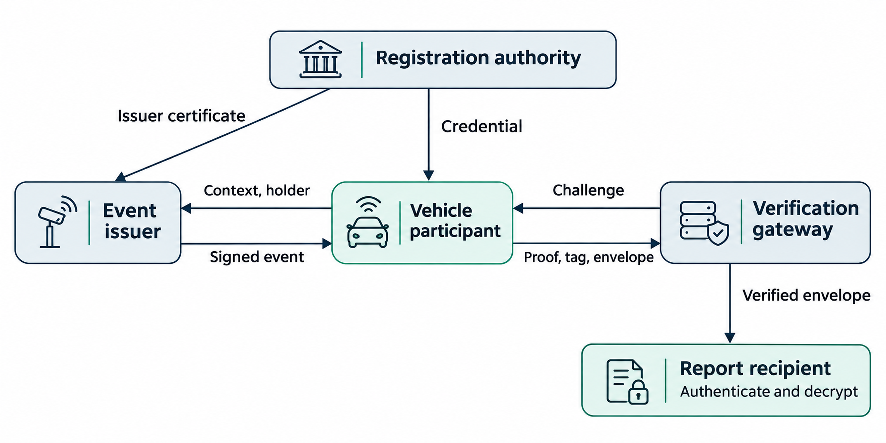
\includegraphics[width=.94\textwidth]{figure1_scientific.pdf}
\caption{Conceptual report-verification workflow. The authority certifies participants and issuers, and the gateway reconstructs the context and verifies the proof. The recipient then authenticates and decrypts the verified envelope. In the tested gateway, these roles are colocated and authentication precedes acceptance.}\label{fig:architecture}
\end{figure*}

\section{System Model and Problem Formulation}
\label{sec:model}

We consider a vehicular crowdsensing task in which each accepted report must be associated with an authorised participant and a spatiotemporal event that satisfies the task policy. The acceptance decision is made at the level of an individual submitted report. A registration authority issues participant credentials and authorises event-evidence issuers. To submit a contribution, a participant prepares a report, obtains an issuer-signed event receipt, and constructs a zero-knowledge proof. A verification gateway then checks the proof and maintains task-specific acceptance state, obtaining the task parameters and the authority's public key from an authenticated configuration. Figure~\ref{fig:architecture} illustrates the system roles and evidence flow.

For a task identifier $\mathsf{id}$, let the policy $P=(\boldsymbol{\ell},\boldsymbol{u})$ define an axis-aligned box over integer coordinates $(x,y,t)$. An event $\boldsymbol z=(x,y,t)$ is eligible when $\ell_j\leq z_j\leq u_j$ holds for each coordinate. The representation and physical meaning of these coordinates are fixed by the application. Our prototype uses unsigned 32-bit coordinates with inclusive bounds, where the first two coordinates represent planar grid coordinates and the third represents a time value. A second circuit variant additionally requires $(x,y)$ to belong to an authorised finite set of grid cells committed by a Merkle root. The verifier configuration is assumed to assign each task identifier to a single immutable box and, in the discrete-region variant, a single root; the prototype snapshots this configuration.

The registration authority is trusted to enrol authorised participants and issuers and to protect its signing key. Likewise, an authorised event issuer is assumed to follow the designated observation procedure when assigning signed event coordinates. By contrast, participants and the communication network may be adversarial: an attacker may substitute reports or receipts, attempt to alter task parameters, submit a proof under a different credential, or replay an earlier submission. The gateway is trusted to apply the configured task and authority parameters, rely on a trustworthy clock, and faithfully maintain its acceptance state. While an issuer's signature authenticates its event assertion and the associated report context, the physical accuracy of that assertion ultimately depends on the issuer's observation procedure.

The issuer and gateway have distinct views of a submission: the issuer observes the event and receives the receipt context, whereas the gateway reconstructs that context to verify the proof. The privacy analysis in Section~\ref{sec:interpretation} considers these views and the information they can reveal when combined.

The intended acceptance condition comprises four requirements: (i) an enrolled participant secret and an authorised issuer support the same receipt; (ii) the signed event satisfies the configured task policy; (iii) the receipt refers to the current task, challenge, and submitted report bytes; and (iv) the participant secret has not previously been used to produce an accepted report for this task. Condition~(iv) enforces uniqueness per credential; interpreting it as a per-person or per-vehicle rule additionally depends on the enrolment policy and on participants not sharing their secrets.

\section{Report-Bound Spatiotemporal Proof}
\label{sec:protocol}

\subsection{Public context and credentials}
\label{sec:context}

Let $\mathbb F$ denote the circuit field, and let $H$ be the field hash function used within the circuit. Domain labels distinguish hash invocations serving different purposes; for clarity, we write $H_d(v_1,\ldots,v_k)=H(d,v_1,\ldots,v_k)$. The registration authority holds a public verification key $A$. Each participant selects a nonzero secret $s$ from a high-entropy distribution and receives an authority signature $\sigma_A$ on $H_{101}(s)$. Similarly, each event issuer holds a verification key $W=(W_x,W_y)$ together with an authority signature $\sigma_W$ on $H_{102}(W_x,W_y)$. In the zero-knowledge proof, the participant secret, both signatures, and the issuer key serve as private witnesses.

To initiate a submission, the gateway issues a fresh challenge $q=(n,e)$ comprising a random nonce $n$ and an expiry time $e$. The participant encapsulates a fresh key to the authenticated recipient using ML-KEM-768~\citep{NIST2024MLKEM}, derives an AES-256-GCM key via HKDF-SHA-256, and encrypts the sensed report into an envelope $R$ that contains both the KEM ciphertext and the authenticated ciphertext. Given the task record $T=(\mathsf{id},\boldsymbol{\ell},\boldsymbol u)$ and the submitted envelope $R$, both parties derive
\begin{align}
 \mathsf{tid}&=\mathsf{TaskField}(\mathsf{id}),\\
 c&=\mathsf{ContextField}(T,q,R),
\end{align}
where the prototype uses SHA-256, domain-separated task encoding, a JSON encoding of the task and challenge, and a SHA-256 digest of the exact submitted bytes; the resulting digests are reduced to field elements. The verifier reconstructs $\mathsf{tid}$ and $c$ from its own task record, its issued challenge and the bytes it receives. Hence neither a participant-selected task policy nor a participant-supplied digest is accepted as the verifier's configuration. Task identifiers must not be reused for a different policy within the same deduplication domain.

Next, the participant computes a context-dependent holder value $h=H_{103}(s,c)$ and presents it to the event issuer as part of the receipt request. Following its event-observation procedure, the issuer signs
\begin{equation}
 m=H_{104}(c,h,x,y,t), \qquad \sigma_E=\mathsf{Sign}_{W}(m).
 \label{eq:receipt}
\end{equation}
Thus, the signed message incorporates both a context-specific value derived from the participant secret and the event coordinates. To apply its own issuance rules, the issuer must receive sufficient authenticated task and challenge information.

\subsection{Proof relation}
\label{sec:relation}

The public instance is $(A,\mathsf{tid},c,N,\boldsymbol{\ell},\boldsymbol u)$, where $N$ denotes the participant's task-scoped tag, and the private witness is $(s,\sigma_A,W,\sigma_W,\sigma_E,x,y,t)$. The proof attests that these values satisfy
\begin{align}
 &s\ne 0, \quad \mathsf{Verify}_A(\sigma_A,H_{101}(s))=1,\label{eq:cred}\\
 &\mathsf{Verify}_A(\sigma_W,H_{102}(W_x,W_y))=1,\label{eq:issuer}\\
 &\mathsf{Verify}_W\!\left(\sigma_E,H_{104}(c,H_{103}(s,c),x,y,t)\right)=1,\label{eq:event}\\
 &N=H_{105}(s,\mathsf{tid}),\label{eq:nullifier}\\
 &0\leq \ell_j\leq z_j\leq u_j<2^{32},\quad j\in\{1,2,3\}.
 \label{eq:policy}
\end{align}
The encoded signing keys must satisfy the curve and subgroup requirements of the underlying signature implementation. Equations~\eqref{eq:cred}--\eqref{eq:event} reuse the same participant secret and context across the credential and event checks. Equation~\eqref{eq:nullifier} then applies that same secret for duplicate detection, while Eq.~\eqref{eq:policy} checks the private event coordinates against the public task bounds. Because the circuit range-constrains both the event coordinates and the policy endpoints prior to comparison, the arithmetic comparison faithfully enforces the stated unsigned integer relation.

\subsection{Discrete region membership}
To support a nonrectangular set of permitted grid cells, the configured verifier constructs a fixed-depth Merkle tree and includes its root $r_{\mathrm{reg}}$ in the public statement. Each valid leaf is computed as $H_{202}(x,y)$, internal nodes are formed as $H_{203}(\mathit{left},\mathit{right})$, and unused leaves are assigned a separate domain label. The participant provides a private authentication path together with Boolean direction bits, enabling the circuit to recompute the Merkle root from the same signed coordinates $(x,y)$ used in Eq.~\eqref{eq:event} and verify its equality with $r_{\mathrm{reg}}$. Our implementation uses a tree depth of eight, accommodating up to 256 distinct authorised coordinate pairs while still enforcing the bounding policy box and time interval. The verifier retrieves $r_{\mathrm{reg}}$ from its trusted task configuration, which binds the task identifier to this immutable root; the root itself is not included in the signed context. Consequently, the membership proof establishes inclusion within the configured discrete cell set, whereas the mapping from physical geography to grid cells remains an external input to policy construction.

The participant submits the tuple $(N,\pi,R,n)$, where $\pi$ is a zero-knowledge proof for the public instance. The report recipient authenticates and decrypts the envelope $R$ using the encapsulated key. In our region-gateway implementation, the gateway also serves as the recipient, verifying both the proof and the ciphertext authentication tag before returning the plaintext. In the research prototype, the signature scheme is EdDSA over the BN254 twisted-Edwards curve, $H$ is MiMC as implemented by the chosen cryptographic library, and the proof system is Groth16 over BN254, with its circuit-specific setup and verification key generated prior to report verification. Under the security assumptions of the proof system, hash function, and signature scheme, the resulting proof verifies the specified relation.

\subsection{Credential-linked identity encryption}
An optional accountability circuit extends the discrete-region relation by incorporating an encrypted registry identity point $I$. Specifically, the registrar signs the binding $\sigma_I=\mathsf{Sign}_A(H_{301}(H_{101}(s),I_x,I_y))$ over the same secret-derived commitment used in Eq.~\eqref{eq:cred}. Let $P_A=[a]B$ denote the auditor's trusted public key in the prime-order group generated by $B$. Sampling a fresh secret scalar $\rho$, the participant computes the ciphertext components $C_1=[\rho]B$ and $C_2=I+[\rho]P_A$. The circuit then additionally verifies both the registrar's binding signature and the two encryption equations using the same secret $s$ that underlies the report credential. While the identity point $I$ and scalar $\rho$ remain private witnesses, $P_A,C_1,C_2$ are included as public proof inputs. The verifier pins $P_A$ and reconstructs the remaining task inputs from its trusted configuration and the received envelope bytes.

Given a verified record, an authorised auditor can recover $I=C_2-[a]C_1$ and resolve the corresponding participant through the registrar's protected identity mapping. Our prototype demonstrates decryption back to the registered group point, whereas authenticating the real-world registry and authorising an identity opening remain external procedural controls. Within the circuit, the proof verifies the correctness of the encryption relation and its binding to the participant credential. This group-based identity encryption operates independently of the ML-KEM report envelope.

\subsection{Active credential membership}
A further circuit extends the accountability relation with a private membership path for the credential currently in use. The registrar maintains a set of active credential commitments $D=H_{101}(s)$. Each occupied leaf is $H_{402}(D)$, nodes use $H_{403}$, and empty leaves use a separate label. The circuit derives $D$ from the same secret as the credential, receipt and task tag and recomputes the configured active-set root along an eight-level private Merkle path. The verifier selects the current root from its trusted configuration. Removing a credential changes the root; a proof generated for the earlier root does not verify against the updated root. The prototype models the sets and root snapshots in memory, with up to 256 credential slots. In the active-set gateway, policy updates and acceptance use the same lock; the instance rejects earlier versions, previously used roots and reinstatement of a credential it recorded as removed. Authenticated root distribution and protection against rollback across restarts are responsibilities of the surrounding configuration service.

\subsection{Gateway acceptance}
\label{sec:acceptance}

Upon receiving a submission, the gateway looks up the unconsumed challenge by its nonce and checks its validity against the local clock. It then reconstructs the public statement from the configured authority, task parameters, stored challenge, received report bytes, and submitted tag. The gateway accepts the submission only if the challenge has not expired, $N$ has not previously been accepted for this task, and proof verification succeeds. In the region-gateway variant, successful ciphertext authentication is also required prior to acceptance and plaintext delivery. A successful acceptance consumes the challenge and records $N$. In the experimental gateway, these state transitions are executed under a single lock, and a failed proof verification does not consume an unexpired challenge. This acceptance state is maintained in memory and applies to a single gateway instance.

Because $N$ depends on the task identifier rather than on the challenge, obtaining a new challenge does not by itself yield a different tag for the same credential and task. Consequently, this rule prevents the gateway from accepting a second contribution bearing the same computed tag within its maintained state. While a fresh challenge binds the receipt to the current submission, it does not by itself guarantee that the underlying sensor measurement was newly captured~\cite{Birkholz2023RATS}.

\subsection{Conditional security and privacy}
\label{sec:interpretation}

\begin{proposition}[Task-scoped single acceptance]
Assume the soundness of the proof relation. For a fixed task identifier and participant secret, if the gateway atomically checks and records the task tag upon each successful submission, it accepts at most one report generated with that secret within its maintained state, up to the soundness error of the proof system.
\end{proposition}
\begin{proof}
Equation~\eqref{eq:nullifier} deterministically maps a fixed participant secret and task identifier to the same tag across all submissions, independently of the challenge. Upon the first successful acceptance, the gateway records this tag. Performing the check and state update atomically prevents any concurrent or subsequent submission carrying the same tag from achieving another successful acceptance within that state.
\end{proof}


\paragraph{Acceptance and receipt binding.} We next consider the base relation under a fixed issuer verification key. Let $M(c,s,\boldsymbol z)=H_{104}(c,H_{103}(s,c),x,y,t)$ denote the receipt message. Before verification, the gateway reconstructs $\mathsf{tid}$ and $c$ from its authenticated task record, stored challenge and received envelope. Given an honestly generated circuit-specific verification key and knowledge soundness, an accepting proof admits an extracted witness satisfying Eqs.~\eqref{eq:cred}--\eqref{eq:policy}, except with the proof system's knowledge-soundness error. The credential, issuer certificate and event receipt therefore verify for the extracted values. As in the system model, the physical correctness of the signed event depends on the issuer's observation procedure.

\begin{proposition}[Conditional reuse of a fixed receipt]\label{prop:receipt-binding}
Fix a nonzero secret $s$, context $c$, event $\boldsymbol z$, issuer key $W$ and issuer receipt $\sigma_E$ that verifies for $M(c,s,\boldsymbol z)$. Suppose the same signature under $W$ cannot be used to authenticate two different field messages, and that collisions in $H_{103}$ and $H_{104}$ are infeasible. An accepting proof that uses this same receipt and issuer key cannot have an extracted witness with a different $(c,s,\boldsymbol z)$, except with the knowledge-soundness error or a violation of one of these assumptions.
\end{proposition}
\begin{proof}
By knowledge soundness, an accepting proof yields a witness satisfying Eq.~\eqref{eq:event}. Signature message binding makes its signed field message equal to $M(c,s,\boldsymbol z)$. If its context, event, or holder value differs from the original, the two different inputs to $H_{104}$ yield the same output, giving a collision. Otherwise, if the context and event agree but the secret differs, equality of the holder values gives a collision in $H_{103}$. The result applies to reuse of the same receipt under the same issuer key. It assumes that the participant secret remains protected and the issuer follows the stated observation procedure; it does not rule out newly issued receipts or relay attacks.
\end{proof}

The reconstructed context also connects the receipt to the received envelope and the current task and challenge. Reusing a receipt with different inputs therefore requires a collision in the concrete context mapping, including its hash-to-field reduction, or a violation of the assumptions in Proposition~\ref{prop:receipt-binding}. The proposition assumes signature message binding and does not constitute a general reduction from EdDSA unforgeability. Cross-task tag privacy is considered separately below.

\paragraph{Role-specific privacy.} The issuer observes the event and receives the context $c$ and holder value $h$ used to issue the receipt. The gateway reconstructs the same $c$ as a public proof input and observes the task, challenge, tag, received envelope and communication metadata. If the issuer and gateway share their records, matching context values can link an event observation to a gateway submission, subject to collisions or ambiguity in those records. A synthetic two-report check confirmed this link in the tested role views. The proof's zero-knowledge property protects its private witnesses, while privacy of the submission also depends on the information available to each role and on whether their records are shared.

The task tag in Eq.~\eqref{eq:nullifier} is deterministic within a task. Its cross-task privacy requires a keyed-hash pseudorandomness assumption for $H_{105}(s,\cdot)$, high-entropy secret generation and appropriate treatment of other observable fields. The circuit checks that $s$ is nonzero; secret entropy is an enrolment assumption rather than a consequence of this check.

\paragraph{Report confidentiality.} In the encrypted-report workflow, the prototype employs ML-KEM-768 key encapsulation, HKDF-SHA-256, and AES-256-GCM with a freshly generated random nonce, authenticating the task identifier as associated data. The zero-knowledge proof binds the resulting ciphertext envelope, rather than the underlying plaintext, to the event receipt. Report confidentiality therefore depends on an authenticated recipient public key, secure key management, and the security assumptions of the KEM and authenticated-encryption schemes, while envelope length and network metadata remain observable. Furthermore, although ML-KEM protects the encapsulated report key, the EdDSA and Groth16 proof components are not post-quantum primitives. Finally, the region gateway verifies ciphertext authenticity before accepting and returning the report.


\section{Evaluation}
\label{sec:evaluation}

We implemented the proposed relation in Go using gnark 0.16.4 and gnark-crypto 0.21.1-0.20260913224755-1409fe592052. All experiments were conducted on an Apple M1 machine equipped with 16 GiB of memory, running macOS 27.2 and Go 1.26.8 (which reported eight logical processors). In the evaluation, the participant, registration authority, event issuer, and gateway were instantiated as in-memory software objects, and all event coordinates and sensing reports were synthetic. Accordingly, the reported measurements characterize the performance of the specified cryptographic operations on this platform.

\subsection{Holder-binding ablation}
To isolate the effect of holder binding, we compare the proposed relation against a bearer-style ablation that retains the exact same credential, issuer-certificate, event, context, bounds, and tag checks, except that the issuer signs a receipt containing a fixed constant in place of $H_{103}(s,c)$.

In this test, two participants held distinct valid credentials and tags while sharing the same task, challenge, report, and event. The attacker was assumed to obtain the victim's receipt, context, and event before the challenge was consumed. Under the full relation, each participant's own receipt satisfied its corresponding witness, whereas substituting the victim's receipt into the attacker's witness caused the constraint solver to fail. Under the bearer ablation, however, the substituted receipt satisfied the circuit and the attacker's resulting Groth16 proof verified successfully. Table~\ref{tab:ablation} illustrates how the holder field binds the receipt to the credential secret in this transfer scenario.

\begin{table}[t]
\centering\caption{Controlled receipt-transfer ablation.}\label{tab:ablation}
\begin{tabular}{@{}lcc@{}}\toprule
Receipt relation & Own receipt & Copied receipt \\\midrule
Holder bound & Accepted & Rejected \\
Bearer control & Accepted & Accepted \\\bottomrule
\end{tabular}\par\vspace{2pt}
\footnotesize The holder-bound cases and the bearer own-receipt case reflect constraint-solver checks, whereas the copied-receipt bearer case also includes a verified Groth16 proof.
\end{table}

\subsection{Context-binding ablation}
Next, we isolate the binding between an issuer-signed event and the corresponding task, challenge, and report. A controlled no-context circuit retains the participant credential, issuer authorization, holder secret, event, and policy checks, but replaces the context in both the holder commitment and the signed receipt with a constant. In this experiment, a single participant reuses a receipt for the same event while substituting one context component at a time. Whereas the full circuit accepts the original context and rejects every substituted witness, the no-context circuit accepts all four cases and produces a verified Groth16 proof for each (Table~\ref{tab:context-ablation}). This comparison isolates the effect of context binding within the tested relation.

\begin{table}[t]
\centering\footnotesize\setlength{\tabcolsep}{3pt}\caption{Controlled context-substitution ablation.}\label{tab:context-ablation}
\begin{tabular}{@{}lcc@{}}\toprule
Test case & Full relation & No context binding \\\midrule
Original context & Accept & Accept \\
Substituted report & Reject & Accept \\
Substituted challenge & Reject & Accept \\
Substituted task & Reject & Accept \\\bottomrule
\end{tabular}\par\vspace{2pt}
\footnotesize Outcomes for the full relation reflect constraint-solver checks, whereas outcomes for the no-context relation additionally include Groth16 proof generation and verification. In all cases, the participant holds the original receipt and a valid credential.
\end{table}

For the holder-binding experiment, we also benchmarked the rectangle circuit alongside its bearer control on the same machine, using an identical task, event, and credential fixture. Each circuit was set up separately and measured across 30 runs following one warm-up run with a fixed valid witness. The holder-bound circuit required 29,833 constraints and generated proofs in $142.67\pm5.48$ ms, compared with 29,173 constraints and $138.35\pm6.65$ ms for the bearer control; proof verification required $1.012\pm0.099$ ms and $0.981\pm0.065$ ms, respectively. These measurements quantify the overhead of the additional holder check in this controlled implementation.

\subsection{Report authentication and replay resistance}
Our proof and gateway tests exercised the complete acceptance relation. A valid Groth16 proof verified successfully against the reconstructed task and report context. Conversely, modifications to the report context, event coordinates, credential secret, signatures, tag, or policy endpoints were all rejected; an honestly signed out-of-policy event was likewise rejected, whereas an event lying directly on the inclusive policy boundaries was accepted. Furthermore, the issuer-key validation tests rejected certified neutral and order-two points, off-curve issuer points, and an off-curve signature point.

At the gateway level, acceptance was bound to the received encrypted envelope and an issued, unexpired challenge, causing modified envelope bytes as well as unknown or expired challenges to be rejected. When two valid submissions carrying different challenges but the same task-scoped tag were submitted concurrently, the single gateway instance accepted exactly one. On the recipient side, valid ML-KEM envelopes were successfully authenticated and decrypted, whereas altered ciphertexts, mismatched task identifiers, and incorrect recipient keys were rejected.

The discrete-region circuit verified proofs for two authorised cells while rejecting altered Merkle paths, direction bits, or signed coordinates, as well as an authorised issuer's signature on a cell outside the configured set and verification attempts against a different root. The accountability circuit verified a valid proof and accurately recovered the bound identity point, while rejecting modifications to the auditor key, ciphertext, identity binding, credential, or tested point and scalar inputs. Finally, the active-set tests confirmed that a proof generated for a removed credential failed against the updated root, whereas a remaining active credential could still prove membership under that updated root.

An integrated gateway test combined active-root updates, report decryption, identity-ciphertext evidence, and task-scoped duplicate checking. In addition, a dedicated concurrency test exercised both deterministic execution orderings and four synchronised races between an active-root update and a report submission. In all cases, the outcomes respected the single-instance serialisation order, and a subsequent proof referencing the old root was rejected after the update without consuming its challenge or task tag. Go's built-in race detector reported no data races across these executions.

\subsection{Proof cost}
The baseline rectangle circuit comprises 29,833 R1CS constraints, encompassing the three signature-verification relations and the spatiotemporal policy checks; the depth-eight discrete-region circuit contains 35,798 constraints, the region-plus-accountability circuit contains 62,627, and the full active-membership circuit contains 68,592. For each of the four circuits, following one warm-up run, we generated and verified 30 proofs using a single setup and a valid synthetic witness per run. Across these runs, the fixture, task, and event were held constant, while the challenge and synthetic report bytes varied. Execution times were measured strictly around the library's proving and verification calls; credential and receipt generation, identity-ciphertext construction and opening, credential-set updates, witness construction, report encryption, network communication, and gateway processing fell outside the timed intervals. Each circuit was compiled and set up once. Table~\ref{tab:cost} reports the sample mean and sample standard deviation across the repeated operations, and Fig.~\ref{fig:bench} plots the individual measurements. All four serialized proofs occupy 164 bytes, while the serialized public witnesses occupy 364, 396, 588, and 620 bytes for the rectangle, region, accountability, and active-membership circuits, respectively. These sizes reflect the proof artifacts alone and are distinct from the complete report submission.

\begin{table*}[t]
\centering\small\caption{Local Groth16 operation costs and serialized sizes.}\label{tab:cost}
\begin{tabular}{@{}lrrrr@{}}\toprule
Quantity & Rectangle & Region & Accountability & Active set \\\midrule
Constraints & 29,833 & 35,798 & 62,627 & 68,592 \\
Compilation (one run), ms & 103.84 & 50.35 & 71.96 & 76.22 \\
Setup (one run), s & 2.596 & 2.182 & 3.204 & 4.424 \\
Proving, ms (mean $\pm$ SD) & $146.74\pm10.53$ & $214.28\pm8.76$ & $303.93\pm12.02$ & $422.47\pm23.72$ \\
Verification, ms (mean $\pm$ SD) & $1.027\pm0.088$ & $0.995\pm0.058$ & $1.056\pm0.257$ & $1.016\pm0.038$ \\
Proof / public witness, bytes & 164 / 364 & 164 / 396 & 164 / 588 & 164 / 620 \\\bottomrule
\end{tabular}
\end{table*}

\begin{figure*}[t]
\centering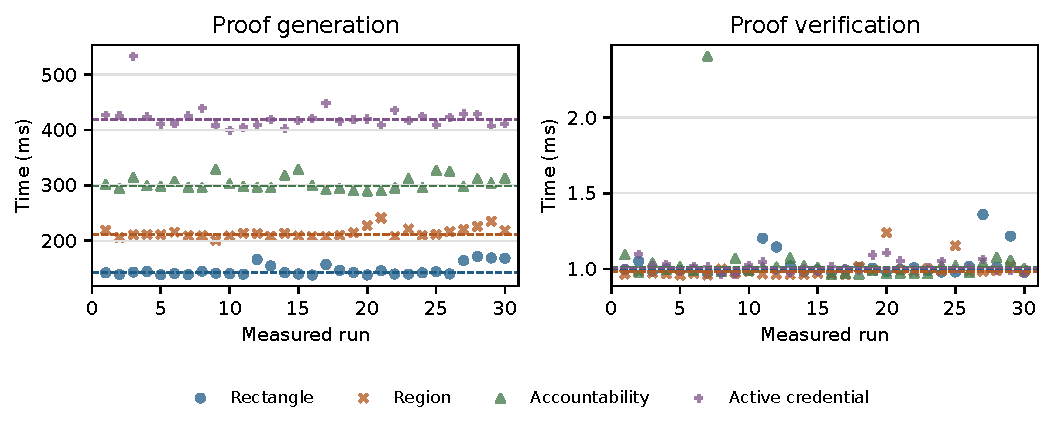
\includegraphics[width=.9\textwidth]{benchmark.pdf}
\caption{Thirty local proof-generation and verification measurements per circuit following one warm-up run. Dashed lines indicate medians; setup, signing, encryption, and network operations are excluded.}\label{fig:bench}
\end{figure*}

\subsection{Effect of region-tree depth}
We next varied the fixed depth of the region-membership circuit while holding the event, task, proof system, and host machine constant. For each depth, a separate circuit and setup were generated, followed by one warm-up run and 30 measured proof executions. At depth $d$, the region tree contained $2^d$ authorised cells, and the participant proved membership for the same cell across all configurations. Table~\ref{tab:region-scaling} reports the resulting sample means and standard deviations. Increasing the tree depth from four to eight adds 2,652 constraints, whereas verification time remains close to one millisecond across these measurements.

\begin{table}[t]
\centering\footnotesize\setlength{\tabcolsep}{3pt}\caption{Region membership cost at different tree depths.}\label{tab:region-scaling}
\begin{tabular}{@{}lrrr@{}}\toprule
Depth / cells & Constraints & Prove (ms) & Verify (ms) \\\midrule
4 / 16 & 33,146 & $206.64\pm8.31$ & $1.004\pm0.023$ \\
6 / 64 & 34,472 & $210.75\pm8.53$ & $1.008\pm0.060$ \\
8 / 256 & 35,798 & $217.29\pm8.88$ & $1.017\pm0.061$ \\\bottomrule
\end{tabular}
\end{table}

\subsection{In-process report workflow}
We also separately benchmarked the complete active-credential workflow within a single process on the same machine. The experiment configured 256 region leaves and 256 active-set entries, of which 31 corresponded to generated test participants and the remainder consisted of synthetic filler digests. Following setup and one warm-up run, 30 distinct test credentials each submitted a single synthetic report under the same task. Each run encompassed challenge issuance, ML-KEM report encryption, fixture-side signature and witness construction, proof generation and serialization, and gateway-side proof verification, authenticated decryption, and duplicate checking. The issuer and registration operations were represented by in-memory software fixtures, with no network transfer or physical sensor measurement involved.

The total elapsed time from challenge issuance to successful gateway acceptance was $410.47\pm17.90$ ms (sample mean $\pm$ sample standard deviation, $n=30$). Within this interval, proof generation accounted for an average of 408.09 ms, report encryption averaged 0.036 ms, fixture signing and witness construction averaged 0.952 ms, and gateway verification, decryption, and duplicate checking together averaged 1.368 ms. Opening the identity ciphertext from an accepted in-memory record was timed separately and averaged 0.336 ms, a figure that excludes independent proof re-verification and registry lookup. Circuit compilation, setup, participant enrollment, key distribution, and network communication fell outside the timed interval.

For a 40-byte synthetic plaintext, the ciphertext envelope occupied 1,158 bytes. The encoded envelope, proof, challenge nonce, task tag and two compressed identity-ciphertext points together occupied 1,482 bytes in the measured representation. This component sum excludes transport framing and configuration distribution; the 620-byte public witness was reconstructed locally for verification rather than included in that sum.

\section{Discussion}
\label{sec:discussion}
Holder binding plays a concrete role in the report-acceptance relation by ensuring that an issuer receipt is verified against the exact credential secret used to derive the task tag. In our controlled transfer scenario, this cryptographic link distinguishes a holder-bound witness from a bearer receipt that could otherwise be reused by another credential holder. Context reconstruction at the gateway then extends this same association to the configured task parameters, the issued challenge, and the received ciphertext envelope.

The four evaluated circuits form a modular progression from basic rectangular policy checks to discrete spatial regions, credential-linked identity encryption, and active-credential membership. Across our implementation, all four variants retain the same 164-byte serialized Groth16 proof size while incrementally adding the constraints and public inputs required for each capability. The complete active-set workflow integrates these circuit checks with encrypted report handling and task-scoped duplicate detection. Throughout, the security guarantees rest on the enrolment, issuer-observation, gateway-state, and cryptographic assumptions detailed in Section~\ref{sec:model} and Section~\ref{sec:interpretation}.

\section{Conclusion}
We presented a report-bound verification relation for vehicular crowdsensing that connects an authorised credential, an issuer-signed spatiotemporal event and the encrypted bytes received for a task. A shared participant secret binds the event receipt to the task-scoped duplicate-detection tag, while the zero-knowledge proof keeps the credential and event coordinates private within the proof under the stated security assumptions. The prototype extends this relation to discrete regions, identity encryption and active-credential membership. Controlled receipt-transfer and gateway tests demonstrate the role of the binding, and local measurements quantify the cost of the proof and complete in-process workflow. The result provides a concrete basis for privacy-preserving acceptance of individual task reports.

\bibliography{references}

\section*{Statements and Declarations}
\noindent\textbf{Funding:} This study received partial support from the Heilongjiang Provincial University Teacher Scientific Research Business Fee (2018-KYYWF0941), the Heilongjiang Provincial Natural Science Foundation Joint Fund Cultivation Project (PL2024F002), the National Foreign Expert Key Support Project (D2O25O185), and the Heilongjiang Provincial Undergraduate University Excellent Young Teacher Fundamental Research Support Plan (YQJH2024239).

\noindent\textbf{Competing interests:} The authors declare that they have no known competing financial interests or personal relationships that could have appeared to influence the work reported in this paper.

\noindent\textbf{Author contributions:} Lili He: supervision. Sheng Jiang: methodology, software, investigation, formal analysis. Shuang Chen: writing -- original draft. Lei Zhang: supervision, corresponding author.

\noindent\textbf{Data and code availability:} The prototype code and the experimental records supporting the findings are provided in the supplementary files accompanying this manuscript.
\end{document}
